
\section{Simulation and Results}
\label{sec:simulation}

In this section we will test the proposed DiSR approach to demonstrate
its effectiveness and to compare it against topology agnostic approach
based on spanning trees and
broadcasting~\cite{Patwardhan05evaluatingthe}, to measure how DiSR
performs in covering the network structure

%\item Against the centralized segment based approach (SR), to evaluate
%if and how its known properties are still preserved in the new nano-scale distributed scenario

\subsection{Nanoxim environment}

In order to quantitatively and qualitatively evaluate the proposed approach a
specific simulation environment has been developed, resulting in
the open source and freely available project called
Nanoxim~\cite{nanoxim}.
Nanoxim is a SystemC tool based on a almost rewritten
version of the Noxim Network-on-Chip simulator~\cite{noxim}. While some
complex features have been removed (e.g. wormhole, congestion/topology
aware routing and selection strategies) new features specifically
taylored for nanoscale scenario were introduced, e.g. the ability to simulate a random
network, the implementation of the DiSR to obtain the segment topology
and the support for defective links and nodes.

%------------------------------------------------------------------------------
\subsection{Experimental setup}
The following parameters have been taken into account when
performing the DiSR simulation:
\begin{itemize}
\item {\emph{Size of the network}}: number of nodes, on a range from
10x10 to 100x100 sized networks. 
%\item {\% defective links}: the probability that each link is
%disconnected or not present, from 0 the amount that yelds
%no more segments.
\item {\emph{\% defective nodes}}: the probability that a node is not
working, thus having all its links cannot be utilized during DiSR setup.  
%Same range as defective links parameter.
\item {\emph{Bootstrap node}}: the node used from upper layer 
to inject the DiSR process. When not explicitly investigating the
impact of each single bootstrap choice, a set representative regions have been
considered, i.e. the central part of the network and the edge corners
\end{itemize}

The show the results, the following evaluation metrics have been adopted:
\begin{itemize}
\item{Node coverage}: this is the fraction of nodes that
are assigned to a segment. In the ideal case, all the non defective
nodes should be assigned, so this metric is useful to show how some
disconnected node regions can negatively impact on the whole DiSR
effectiveness.
\item{\emph{Latency}}: this measures how the cycles required to complete the
segment assignment scales for increasing network sizes and defect rates
\item{\emph{Bootstrap node effect}}: this evaluates the impact of the chosen
bootstrap node on the node coverage.
\end{itemize}

%Further, to evaluate how DiSR compares against the centralized segment
%based algorithm, the following metrics have been adopted:
%\begin{itemize}
%%\item {Average Path Lenght}:
%%\item {Average Link Weight}:
%\item {Unidirectional restrictions:}
%\item {Number of Segments}:
%\end{itemize}

Since the distribution of defects and thus the resulting topology is randomly
generated, a set of simulations with different seeds has been run
for each system configuration. We found that 20 repetitions are
required in order to obtain statistically significant results.

% TODO: long paper
\subsection{Other Optimisations}
Some optimisation parameters, which demostrated to improve the DiSR
results have been fixed to some good values, but are not subject to
further investigation; once again the focus here is not the
optimal set of segments, but just demostrating a working approach. 
These are optimisations are:
\begin{itemize}
\item{cycle\_links}: max number of retries across the set of links of
each node. While searching for a free link due an incoming request,
the same request is cancelled after a given number of tries. This
gives to preceding node change to test a different paths. Default is set to 1.
\item{bootstrap\_timeout}: number of time units that a bootstrap node
should wait before assuming that a livelock in the starting segment
process has occurred. In the worst case, we can imagine that longest
path required is the one returning to the bootstrap node after having
travelled across all the links. So, althought this is just an extreme
situation, a good upper limit can be safely be set to NxN.
\item{bootstrap\_immunity}: in order to avoid the failure of the whole DiSR
setup process, a bootstrap node should not have defective links.
Enabling this optimisation, a bootstrap node is immune to defects.
We may think of a pre-bootstrap phase that properly selects (from upper
layer via) a bootstrap node which is tested as properly connected. We
enabled this optimisation, however empirical tests showed us that only
simulations using bootstrap nodes placed on edges would be heavily
affected, since these are nodes starting with a lower number of links,
e.g. corner nodes could only have two connected direction, so even a
defective link could prevent starting segment packet to return to
bootstrap to close the loop a create the segment.
\end{itemize}

\subsection{Results}
\label{sec:results}

In this section we analyze the results in terms of node
coverage and latency at different network sizes, defect rates and
bootstrap injection points.  In particular
Figure~\ref{fig:results_coverage} shows
node coverage for DiSR and RPF tree based approach respectively. While
the first aim of DiSR is not to reach the optimal coverage, we still
can observe a quite good performance as compared to the tree based
approach. Note that defect rates beyond 25\% lead to many disconnected
regions of nodes that DiSR currently cannot handle.
For example Figure~\ref{fig:net} show a 30x30 network with a 25\%
defect in which the bottom-left part cannot be reached due
disconnected regions. Note that remaining defective nodes belonging to
connected regions are successfully surrounded by DiSR coverage; in any
case, these defect levels should be considered as worst case scenarios, so the
achieved coverage of $0.5$ is a satisfying result for this first
version of DiSR. On the other hand, the network size seems to have a
limited impact when defect rate do not introduce too much disconnected
regions. 
\begin{figure}
\centering
\begin{tabular}{cc}
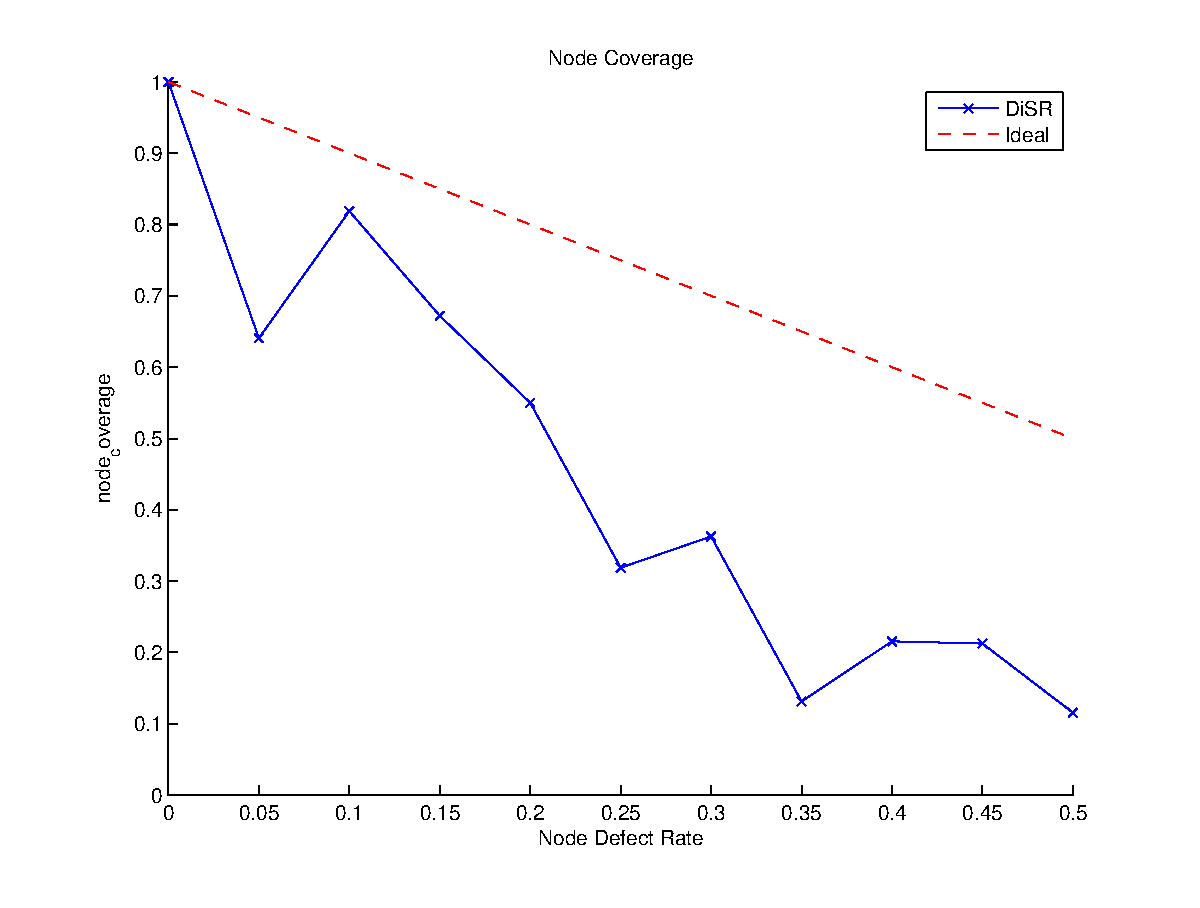
\includegraphics[width=0.48\textwidth]{pictures/set1.eps} & 
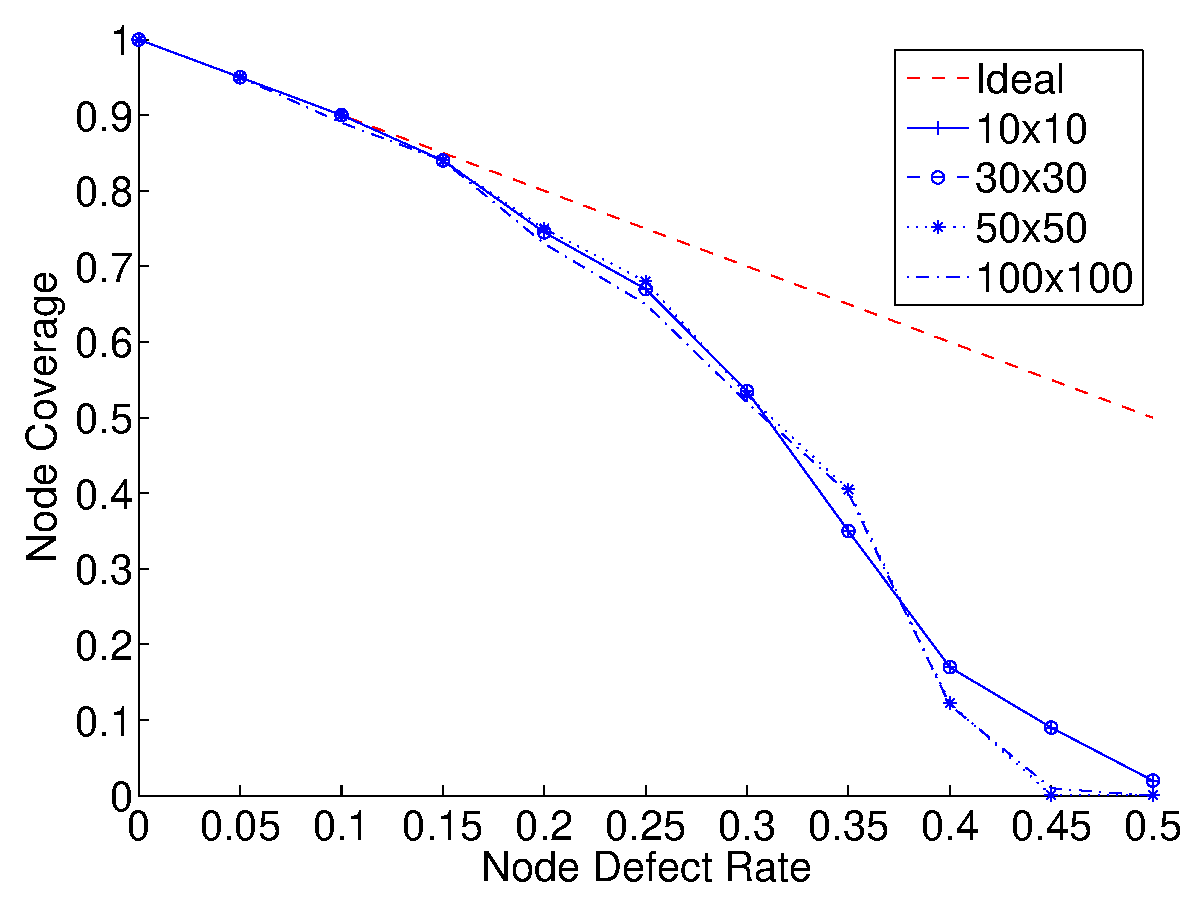
\includegraphics[width=0.48\textwidth]{pictures/coverage.eps} \\
(a) & (b) 
\end{tabular}
\caption{DiSR (a) and RPF (b) node coverage}
\label{fig:results_coverage}
\end{figure}

\begin{figure}
\centering
\includegraphics[width=0.70\textwidth]{pictures/net.ps}
\caption{Covered regions in a 30x30 network with 25\% defects}
\label{fig:net}
\end{figure}

\begin{figure}
\centering
\begin{tabular}{cc}
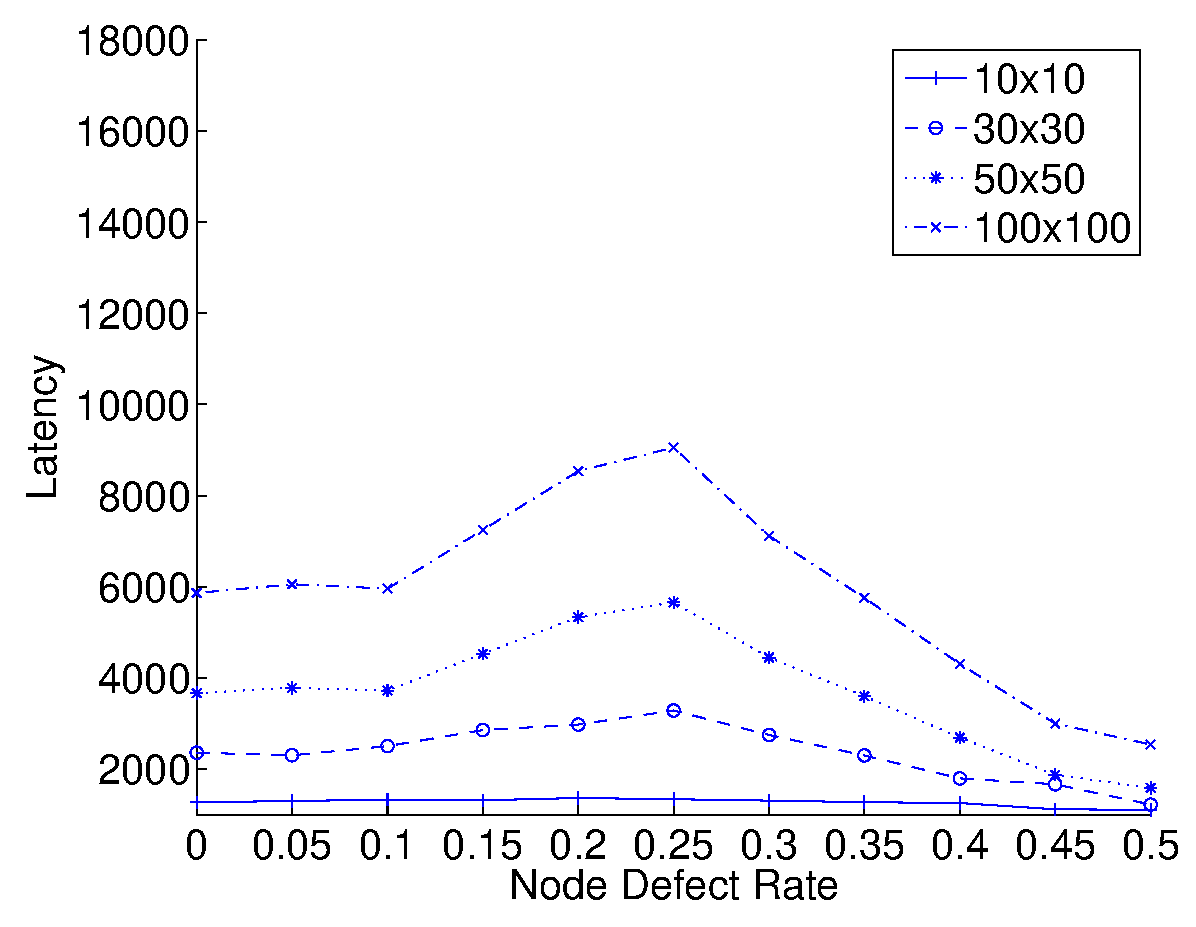
\includegraphics[width=0.48\textwidth]{pictures/set2.eps} & 
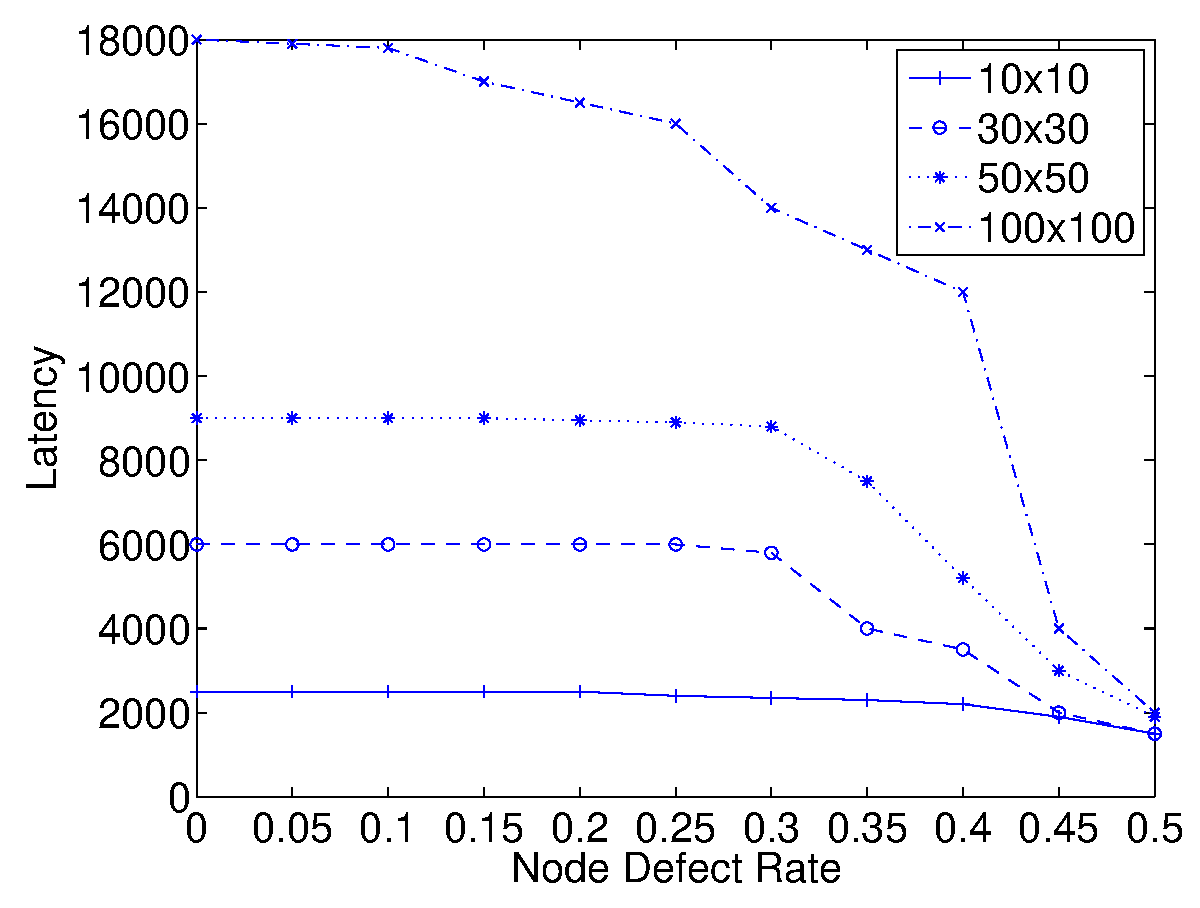
\includegraphics[width=0.48\textwidth]{pictures/set2_rpf.eps} \\
(a) & (b)
\end{tabular}
\caption{Latency of DiSR (a) vs tree based RPF (b) }
\label{fig:results_latency}
\end{figure}

The number of cycles required to complete segment mapping process
is shown in Figure~\ref{fig:results_latency}. In this case comparison
against tree-based shows better (lower) values at different defect
rates.  Rather than the absolute numbers, what it's more interesting
to observe is how DiSR latency scales with network size. For example,
going from 900 to 2500 nodes, at the medium defect rate of $0.15$,
leads to an increase from 3000 to 4500 cycles. It should be noticed
also how the effect of defect rate is increasing until the threshold
of $0.25$ is reached, meaning that until that limit DiSR finds it more
and more difficult to complete the process due increasing defective
paths, but still discover new segments when let running for a more
extended amount of cycles. This behavior is not reported in the RPF
based approach, meaning that a tree based approach, although starting
from higher values, is less affected by defect rates (when low rates
are considered).
After the $0.25$ threshold, the impact of entire disconnected regions
becomes predominant and both approaches become faster in completing
the covering process, since far less nodes can be actually reached. 

Finally, Figure~\ref{fig:results_bootstrap} visually represents  the
stability of the approach against choices of a different bootstrap
node in a 10x10 network.  This is an important aspect to evaluate when
considering that one of the main advantages of DiSR against all the
tree based approaches should be the ability of choosing whatever
bootstrap node, without having to care about the role assumed in the
future by the chosen root node.  In other words, after segments have
been established, the bootstrap node is like every other node, i.e. it
is not center of a structure, and it is not an hotspot for the traffic
distribution. The results in terms of coverage,  shown for low, medium
and high defect profiles, demonstrate a relatively limited
impact of the bootstrap choice in the low/medium scenarios, while a
$30\%$ instability is found for very high defect rates. This also
sounds acceptable, since when a lot of defective nodes are present, the
particular position of the bootstrap node could lead to a completely
different evolution in the DiSR setup process.

\begin{figure}
\centering
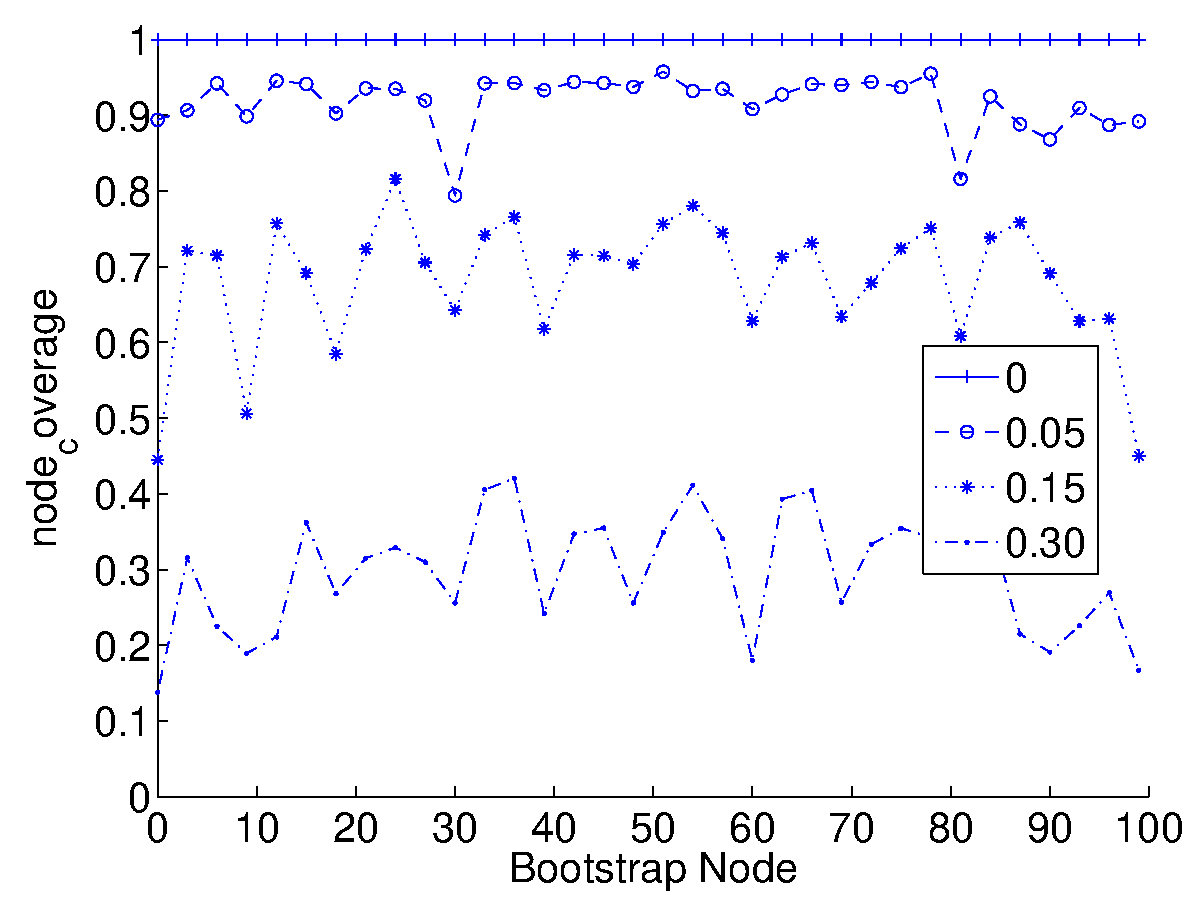
\includegraphics[width=0.48\textwidth]{pictures/set3.eps}
\caption{Effect of bootstrap node}
\label{fig:results_bootstrap}
\end{figure}

